\documentclass[a4paper,11pt]{report}
\usepackage[french]{babel}
\usepackage[T1]{fontenc}
\usepackage[utf8]{inputenc}
\usepackage{lmodern}
\usepackage{microtype}
\usepackage{hyperref}
\usepackage{tabulary}
\usepackage{framed}
\usepackage{fancyhdr}
\usepackage{amsmath}
\usepackage{bbm}
\usepackage{graphicx}
\usepackage{version}

\newcommand{\latin}[1]{\textit{#1}}

\usepackage{anysize}
%left,right, top, bottom
\marginsize{0.8in}{0.8in}{0.8in}{0.8in}


\pagestyle{empty}

\pagestyle{fancy}
\fancyhead{}
\renewcommand{\headrulewidth}{0.5pt}
\fancyhead[L]{\textit{\nouppercase{\leftmark}}}
\fancyfoot{}
\renewcommand{\footrulewidth}{0.5pt}
\fancyfoot[R]{\thepage}

\begin{document}
	\begin{titlepage}
		\vspace*{\stretch{2}}
		\begin{center}
			\large\bfseries\itshape Projet SF\\
		\end{center}
		\noindent\rule{\linewidth}{3pt}

		\begin{center}
			\Huge\bfseries\itshape RAPPORT\\
		\end{center}
		
		\noindent\rule{\linewidth}{3pt}
		\begin{center}
			\bfseries
			\large Modèlisation et Vérification du comportement de véhicules automatiques\\sur un pont à voie unique
			
		\end{center}
		\vspace*{\stretch{2}}
		\begin{center}
			Réalisé par \bfseries \itshape DOAN Cao Sang
		\end{center}
		\begin{center}
			\today
		\end{center}
	\end{titlepage}

\chapter{Propriétés}
	{\huge \itshape L}e programme doit satisfaire les propriétés suivantes:
		\begin{enumerate}
			\item \textit{Il n'y a pas de collision (i.e. deux véhicules circulants en sens inverse) sur le pont.}
			\item \textit{Un véhicule qui arrive est certain de passer sur le pont à l'issue d'une durée bornée.}
		\end{enumerate}
	
\chapter{Explication}
	Je me constate que les jetons colorés ne sont pas bien exporter en format CAMI, par exemple, dans le modèle \textit{Controlleur(CTRLP)} la place \textbf{Budget}, domain \textbf{TimeOut}, j'ai initialisé avec le jeton \textit{<TimeOut.3>} mais quand j'exporte en format CAMI et ré-importe, cette place est initialisée avec un jeton \textit{<3>}. Du coup, les formules CTL ne marche pas car le coloane ne connaît pas le jeton \textit{<3>}. Donc, j'ai mis à côté des fichiers CAMI, des fichiers du type \textbf{.model}, grâce à ces fichiers vous pouvez importer directement le modèle (dans le coloane, \textbf{Import} $\rightarrow$ \textbf{File system}). En plus, j'ai mis aussi mon répertoire entier dans lequel je travaille pour vous faciliter votre travail (sous Mac). Merci de votre attention.
\section{Question 1.1}
\subsection{Vaa}
	\begin{description}
		\item[VerificationA] est une \texttt{place} de sortie, qui lie le composant \textit{Vaa} avec le contrôlleur \textit{CTRLP}, lorsque un véhicule A veut traverser le pont, d'abord il communique avec le contrôlleur \textit{CTRLP} pour avoir son autorisation.
		\item[OKControlleurA] est une \texttt{place} d'entrée qui lie entre \textit{Vaa} et \textit{CTRLP}, lorsque le \textit{Vaa} peut traverser sur le pont, le \textit{CTRLP} met son jeton pour que \textit{Vaa} puisse passer.
		\item[OKPont] est une \texttt{place} entrée qui lie le \textit{P} avec le \textit{Vaa}, le \textit{P} marque cette place lors qu'il reçoit l'autorisation de contrôlleur \textit{CTRLP}.
		\item[AuRevoirControlleurA] est une \texttt{place} de sortie, le \textit{Vaa} marque cette place dès qu'il sort du \textit{P}.
	\end{description}	
	
	\subsection{Vab}
	\begin{description}
		\item[VerificationB] est une \texttt{place} de sortie, qui lie le composant \textit{Vab} avec le contrôlleur \textit{CTRLP}, lorsque un véhicule B veut traverser le pont, d'abord il communique avec le contrôlleur \textit{CTRLP} pour avoir son autorisation.
		\item[OKControlleurB] est une \texttt{place} d'entrée qui lie entre \textit{Vab} et \textit{CTRLP}, lorsque le \textit{Vab} peut traverser sur le pont, le \textit{CTRLP} met son jeton pour que \textit{Vab} puisse passer.
		\item[OKPont] est une \texttt{place} d'entrée qui lie le \textit{P} avec le \textit{Vab}, le \textit{P} marque cette place lors qu'il reçoit l'autorisation de contrôlleur \textit{CTRLP}.
		\item[AuRevoirControlleurB] est une \texttt{place} de sortie, le \textit{Vab} marque cette place dès qu'il sort du \textit{P}.
	\end{description}	
	
	\subsection{Pont}
	\begin{description}
		\item[CapaciteControlleur] est une \texttt{place} de sortie, qui lie le composant \textit{P} avec le contrôlleur \textit{CTRLP} pour lui signaler sa capacité restante.
		\item[OKPont] est une \texttt{place} de sortie qui lie le \textit{P} avec les 2 composants \textit{Vaa} et \textit{Vab}, le \textit{P} marque cette place lorsque sa capacité reste suffisante.
	\end{description}	
	
	\subsection{CTRLP}
	\begin{description}
		\item[VerificationA] est une \texttt{place} d'entrée, qui lie le composant \textit{Vaa} avec le contrôlleur \textit{CTRLP}, lorsque un véhicule A veut traverser le pont, le \textit{CTRLP} doit d'abord, recevoir sa demande.
		\item[VerificationB] est une \texttt{place} d'entrée, qui lie le composant \textit{Vab} avec le contrôlleur \textit{CTRLP}, lorsque un véhicule B veut traverser le pont, le \textit{CTRLP} doit d'abord, recevoir sa demande.
		\item[OKControlleurA] est une \texttt{place} de sortie qui lie entre \textit{Vaa} et \textit{CTRLP}, lorsque le \textit{Vaa} peut traverser sur le pont, le \textit{CTRLP} met son jeton pour que \textit{Vaa} puisse passer.
		\item[OKControlleurB] est une \texttt{place} de sortie qui lie entre \textit{Vab} et \textit{CTRLP}, lorsque le \textit{Vab} peut traverser sur le pont, le \textit{CTRLP} met son jeton pour que \textit{Vab} puisse passer.
		\item[CapaciteControlleur] est une \texttt{place} d'entrée, qui lie le composant \textit{P} avec le contrôlleur \textit{CTRLP} pour savoir la capacité restante du \textit{P}.
		\item[AuRevoirControlleurA] est une \texttt{place} d'entrée, cette place est marqué par le \textit{Vaa}.
		\item[AuRevoirControlleurB] est une \texttt{place} d'entrée, cette place est marqué par le \textit{Vab}.
	\end{description}	
	
\section{Question 1.2}
	Cette composant contient 8 places, dont 4 ont pour le rôle d'interface, et 3 transitions.
	
	La place \textbf{VehiculeA} modélise le véhicule A  lors qu'il arrive devant le pont. S'il veut passer sur le pont, d'abord, il communique avec le contrôlleur par la transition \textit{demanderEntrerA}, cette transition met un jeton dans l'interface \textbf{VerificationA} qui lie avec le contrôlleur \textit{CTRLP} et passe à l'état \textbf{AttenteAutorisationA}. Lorsqu'il reçoit l'autorisation du contrôlleur \textit{CTRLP} via l'interface \textbf{OKControlleurA} et celle du pont \textit{P} via l'interface \textbf{OKPont}, il peut traverser le pont, en passant à l'état \textbf{DansPontA}. Ensuite, quand il sort, il marque la place d'interface \textbf{AuRevoirControlleurA} et aussi passe à l'état \textbf{FiniA} par la transition \textit{sortPontA}.
	
	La sécurité est garantie car, pour passer à l'état \textbf{AttenteAutorisationA} le véhicule doit d'abord communiquer avec le contrôlleur \textit{CTRLP}. Pour entrer, il doit avoir l'autorisation du contrôlleur \textit{CTRLP} et consommer le jeton dans la place d'interface \textbf{OKPont},  cette place modélise la consommation de la capacité du pont \textit{P}. Enfin, il signale sa sortie du pont au contrôlleur \textit{CTRLP} en mettant un jeton dans la place \textbf{AuRevoirControlleurA}.

	\begin{figure}[!htbp]
		\centering
		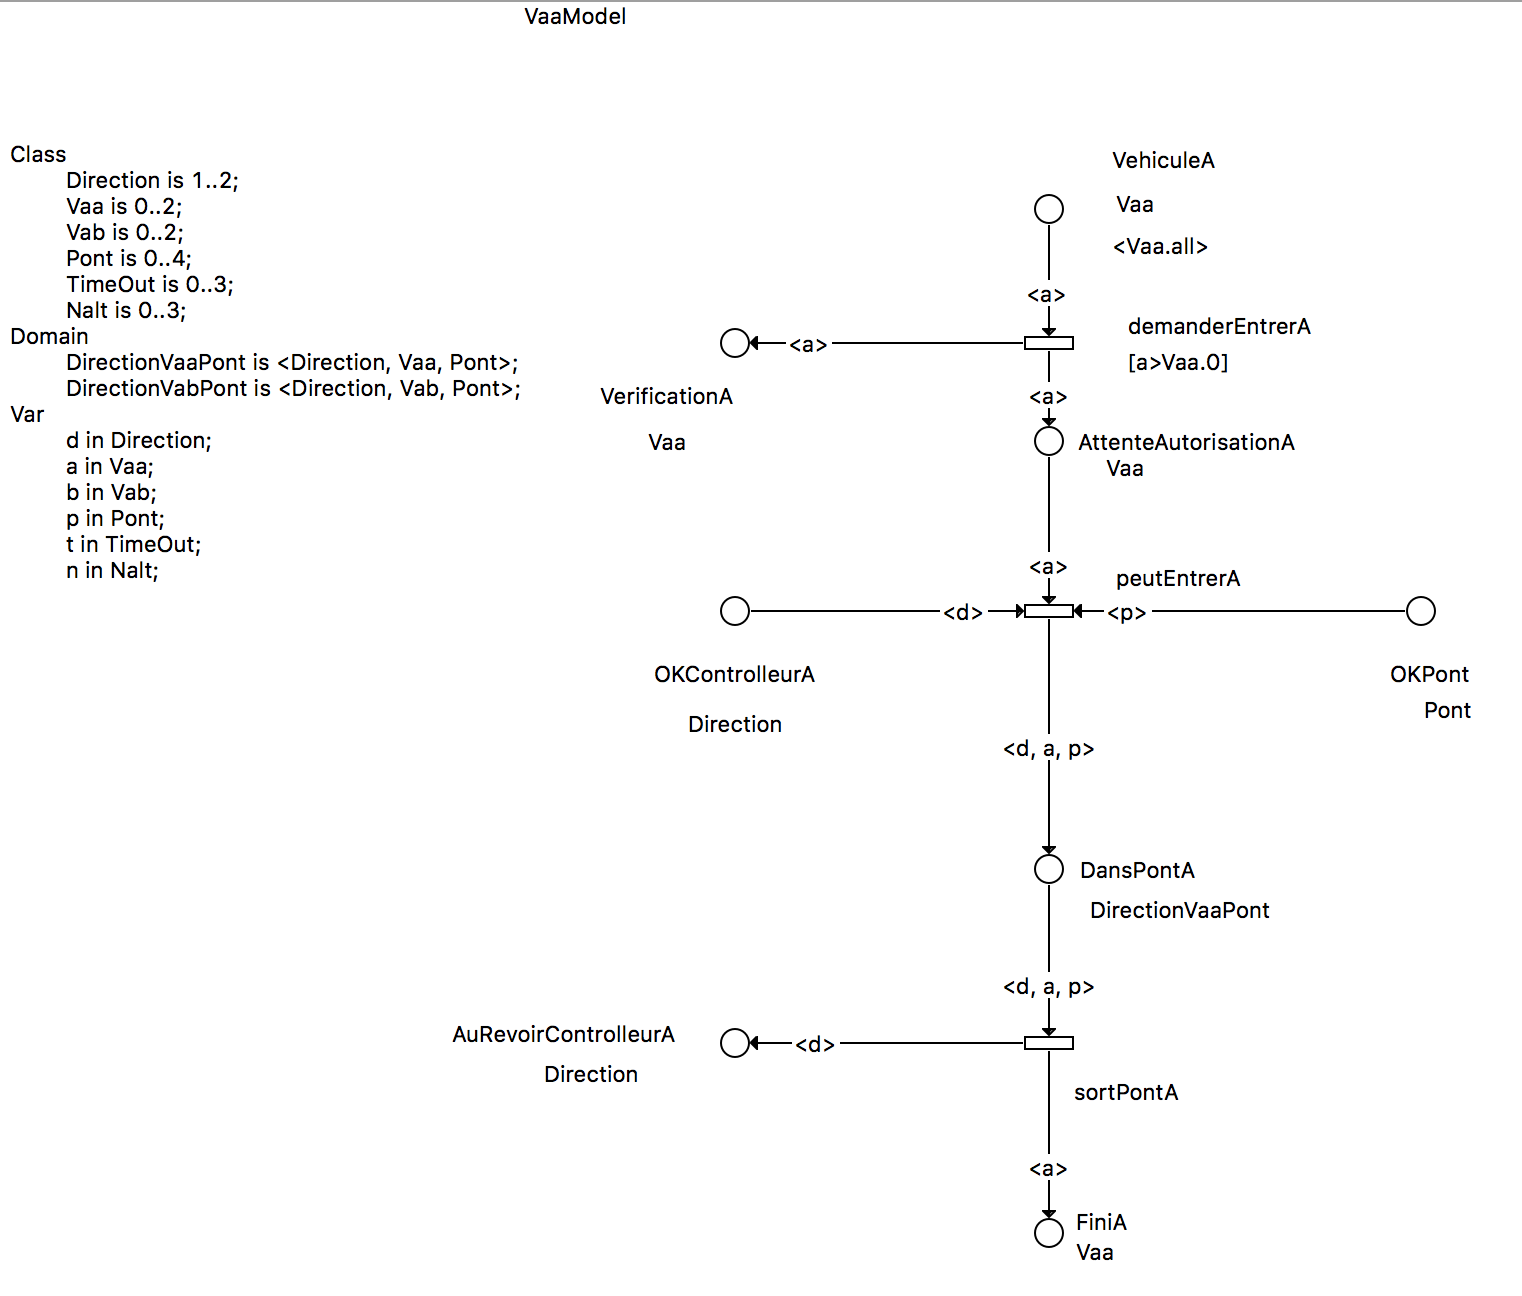
\includegraphics[width = 15cm]{vaaModel.png}
		\caption{Le composant modélise le véhicule automatisée A.}
	\end{figure}
	\newpage
	
\section{Question 1.3}
	Cette composant est identique avec celle de véhicule A, contient 8 places, dont 4 ont pour le rôle d'interface, et 3 transitions.
	
	La place \textbf{VehiculeB} modélise le véhicule B  lors qu'il arrive devant le pont. S'il veut passer sur le pont, d'abord, il communique avec le contrôlleur par la transition \textit{demanderEntrerB}, cette transition met un jeton dans l'interface \textbf{VerificationB} qui lie avec le contrôlleur \textit{CTRLP} et passe à l'état \textbf{AttenteAutorisationB}. Lorsqu'il reçoit l'autorisation du contrôlleur \textit{CTRLP} via l'interface \textbf{OKControlleurB} et celle du pont \textit{P} via l'interface \textbf{OKPont}, il peut traverser le pont, en passant à l'état \textbf{DansPontB}. Ensuite, quand il sort, il marque la place d'interface \textbf{AuRevoirControlleurB} et aussi passe à l'état \textbf{FiniB} par la transition \textit{sortPontB}.
	
	La sécurité est garantie car, pour passer à l'état \textbf{AttenteAutorisationB} le véhicule doit d'abord communiquer avec le contrôlleur \textit{CTRLP}. Pour entrer, il doit avoir l'autorisation du contrôlleur \textit{CTRLP} et consommer le jeton dans la place d'interface \textbf{OKPont},  cette place modélise la consommation de la capacité du pont \textit{P}. Enfin, il signale sa sortie du pont au contrôlleur \textit{CTRLP} en mettant un jeton dans la place \textbf{AuRevoirControlleurB}.

		\begin{figure}[!htbp]
		\centering
		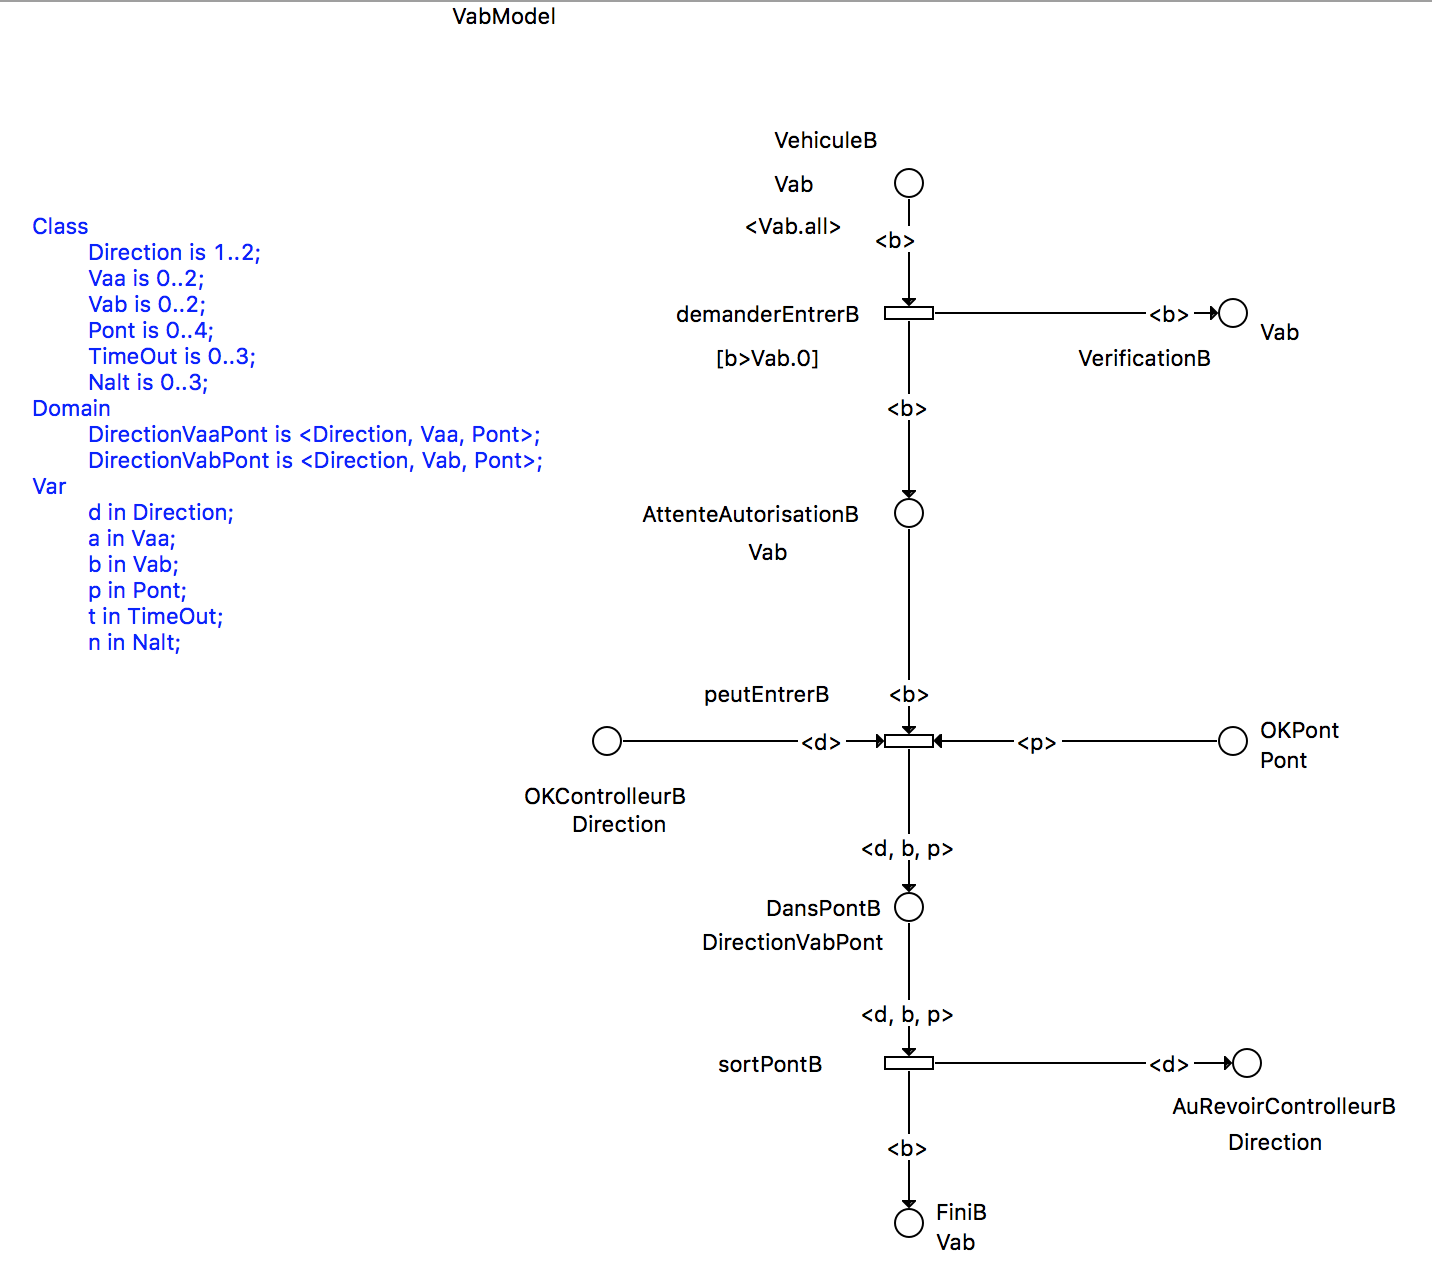
\includegraphics[width = 15cm]{vabModel.png}
		\caption{Le composant modélise le véhicule automatisée B.}
	\end{figure}
	\newpage
	
	
\section{Question 1.4}
	Le comportement d'un pont est simple, il notifie  sa capacité au contrôlleur \textit{CTRLP} et diminue si consommé par un véhicule. Donc, il contient 3 places, dont 2 interfaces et une transition.
	
	La transition \textit{notifieCapacite} marque 2 interfaces \textbf{CapaciteControlleur} et \textbf{OKPont} par 2 jetons, 1 pour chaque.

	\begin{figure}[!htbp]
		\centering
		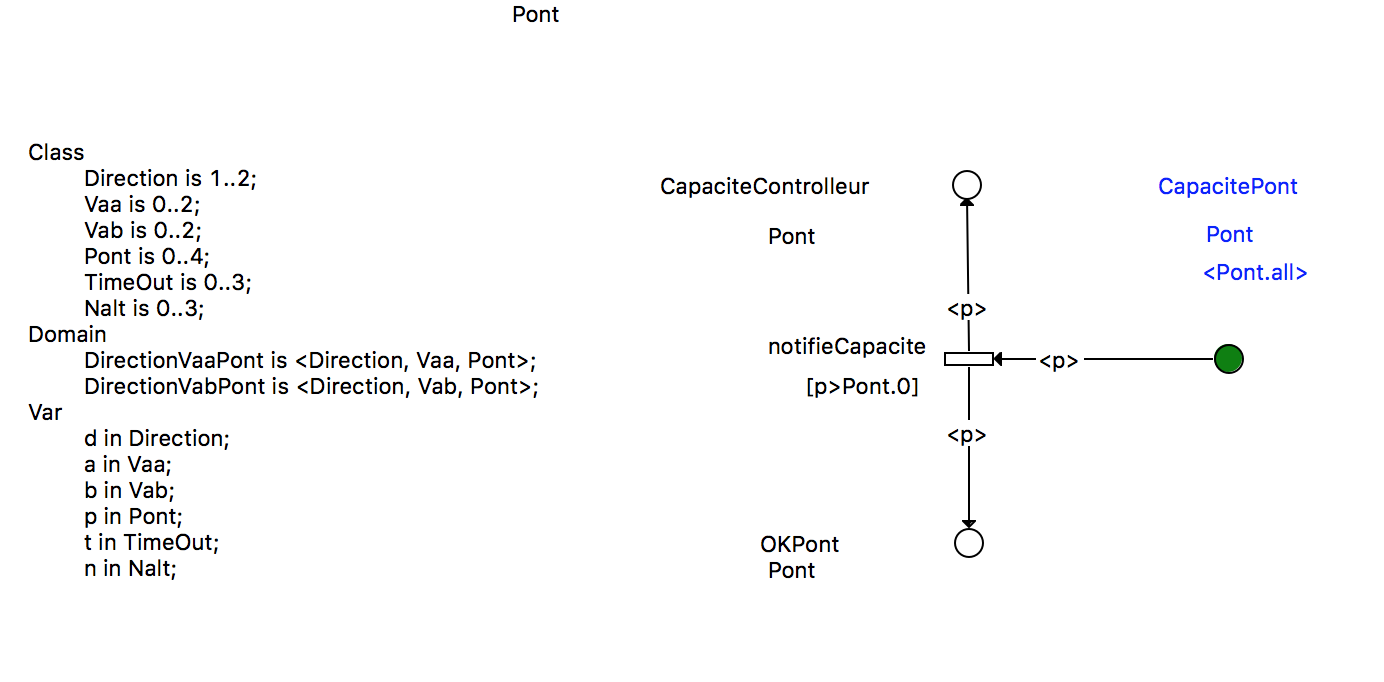
\includegraphics[width = 15cm]{pontModel.png}
		\caption{Le composant modélise le pont.}
	\end{figure}
	\newpage
	
\section{Question 1.5}
	Ce composant contient 12 places dont 7 interfaces, et 6 transitions.
	
	Lorsque le \textit{CTRLP} reçoit une demande d'entrer d'une véhicule \textit{Vaa} (idem, \textit{Vab}) via l'interface \textbf{VerificationA} (idem. \textbf{VerificationB}), il vérifie le sens actuel (initilisé à 1, direction de A vers B) est correspondant à celui de \textit{Vaa} (idem, \textit{Vab}), le timeout restant, le nombre \textit{Nalt} restant et la capacité \textit{CapaP} restant du pont. Si ces conditions sont satisfaites, alors le contrôlleur \textit{CTRLP} donne l'autorisation au véhicule \textit{Vaa} (idem, \textit{Vab}) en attente. Quand le véhicule sort du pont, le contrôlleur reçoit son signal. 
	
	Le timeout est modélisé par une place nommée \textit{TimeOut} avec une seule transition \textit{ecoule}. Le \textit{TimeOut} décrémente une unité de temps automatiquement et indépendamment avec le système. Lors de l'expiration de \textit{TimeOut}, il réinitialise le \textit{Nalt}, lui même, et change la direction actuelle.  Idem pour le \textit{Nalt}, si \textit{Nalt} = 0, il réinitialise le \textit{TimeOut}, \textit{Nalt} et change la direction.
	
	Quand la capacité du pont est à 0, alors aucun véhicule ne peut utiliser ce pont.

	\begin{figure}[!htbp]
		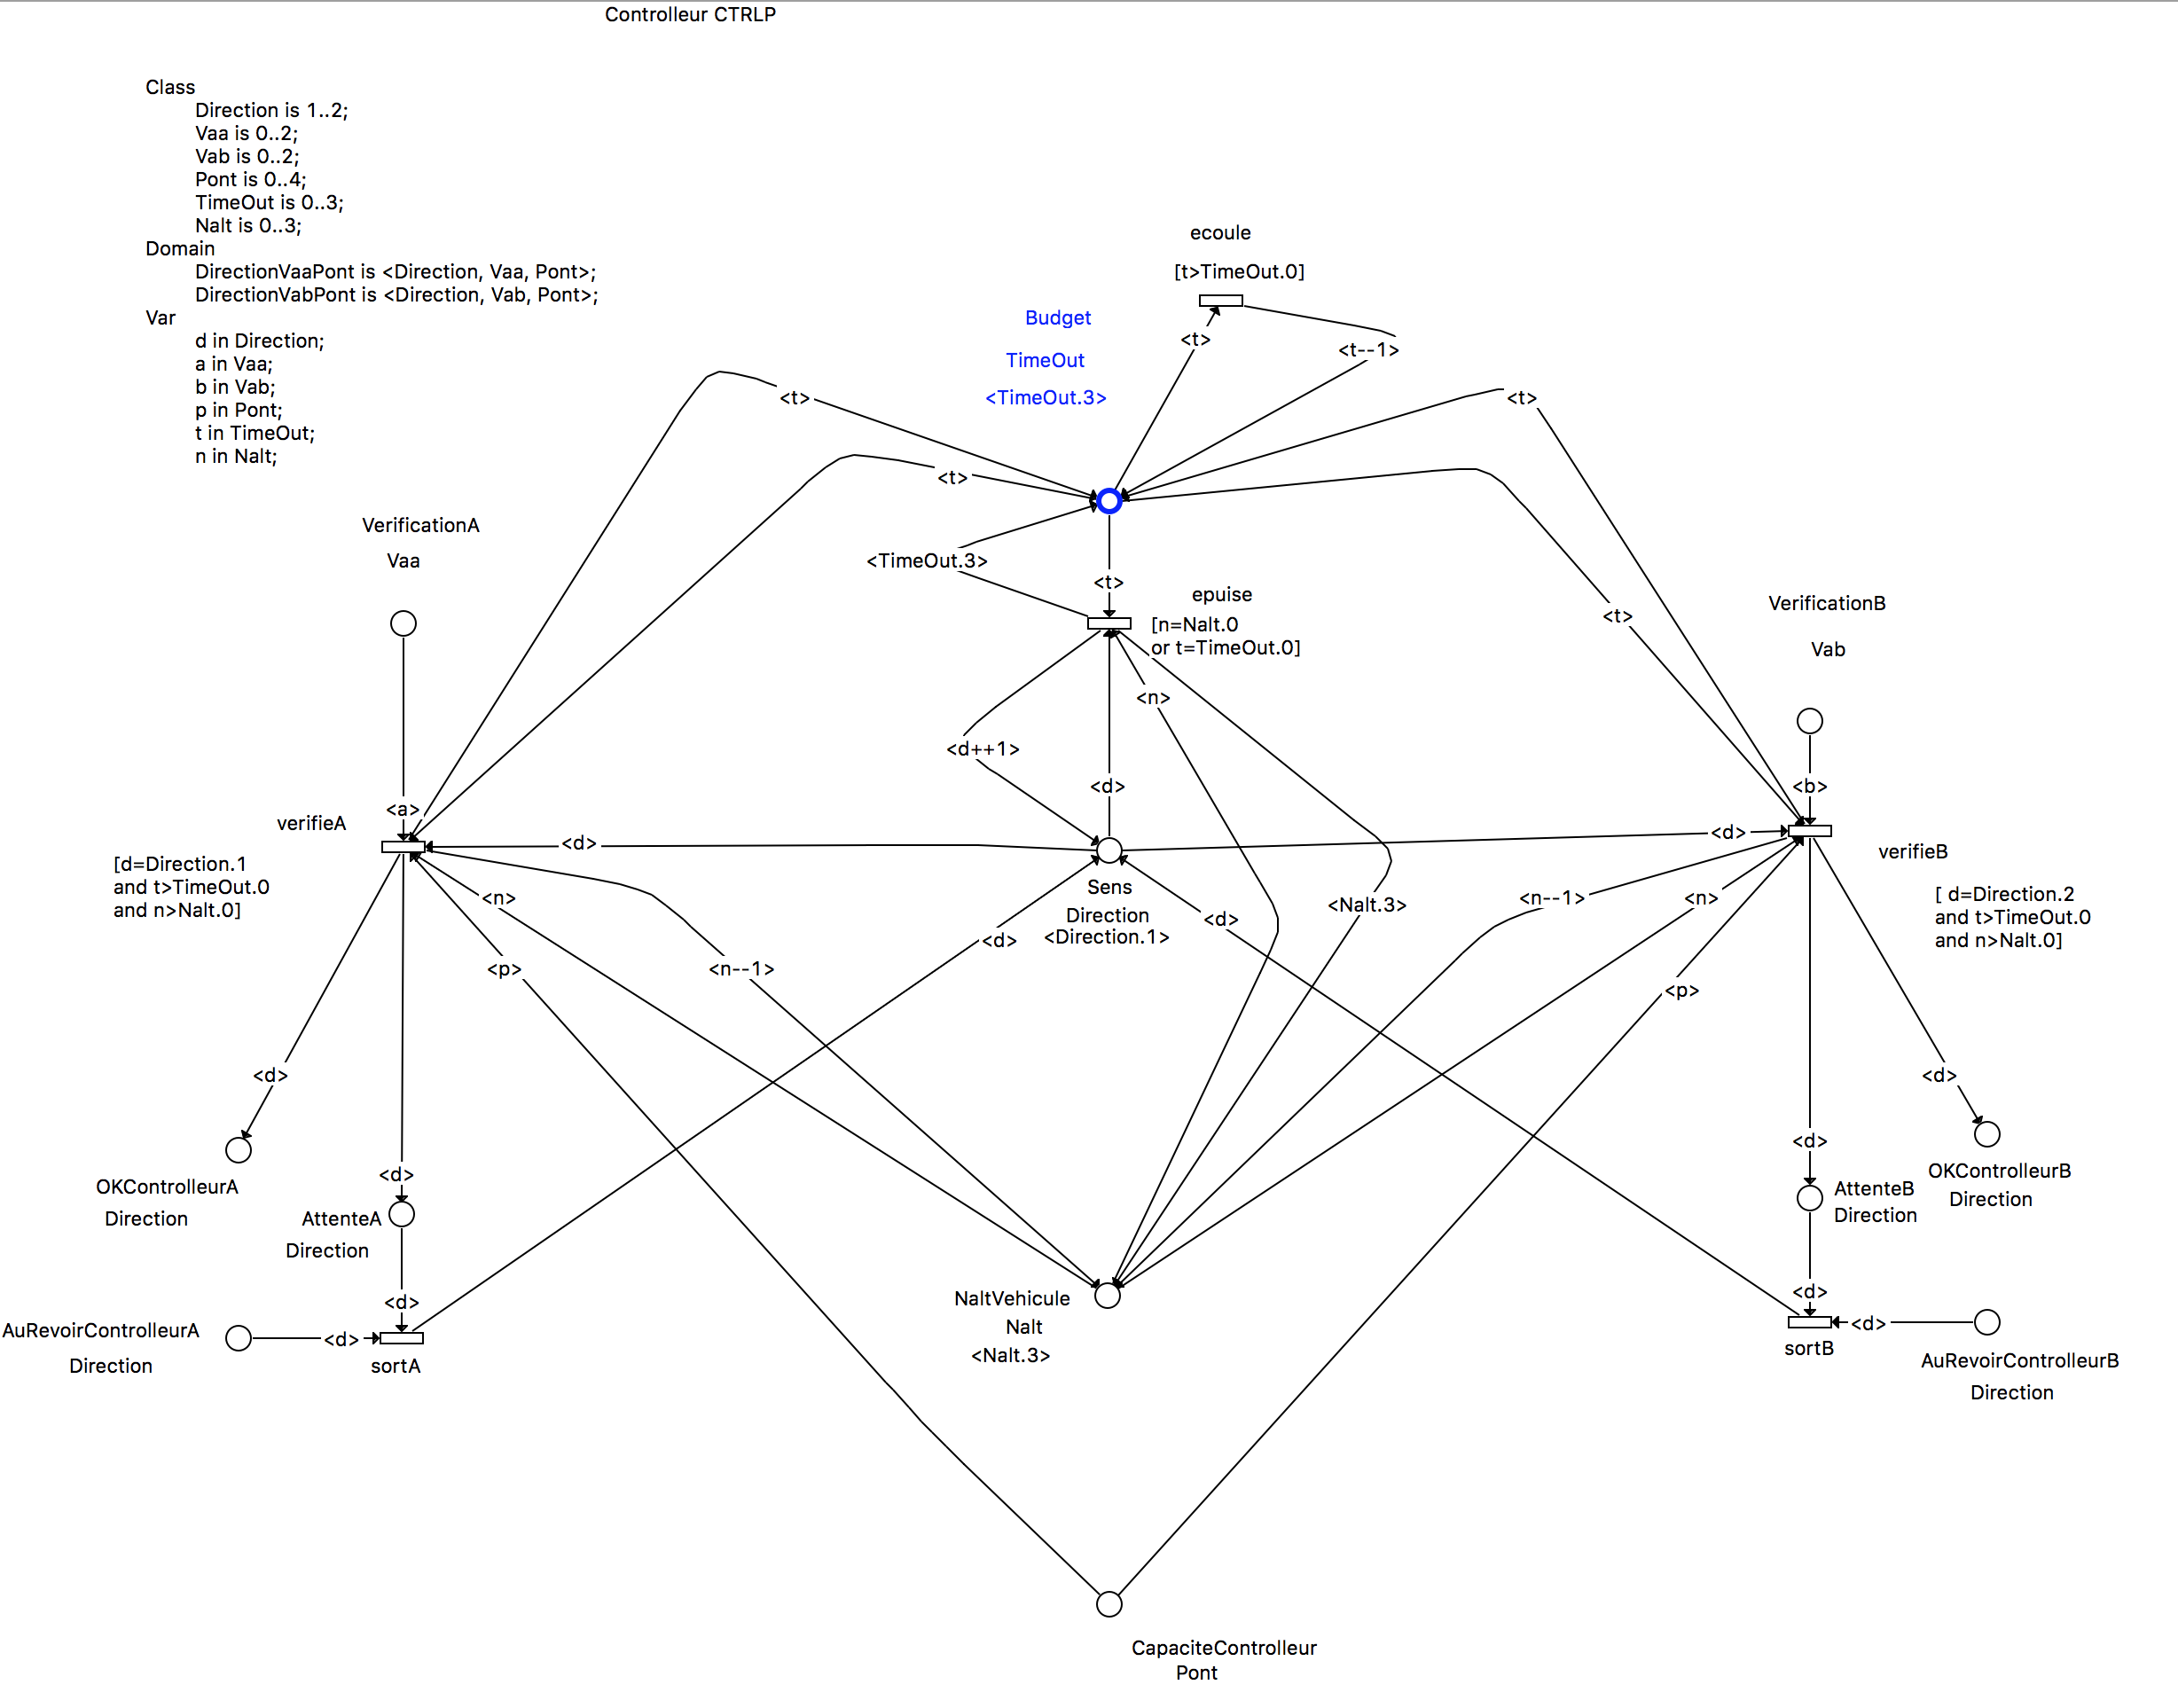
\includegraphics[width = 18cm]{ctrlpModel.png}
		\caption{Le composant modélise le pont.}
	\end{figure}
	\newpage
	
\section{Question 1.6}
	Cette assemblage contient 22 places, 13 transitions et 55$  $ arcs.
	
	Les propriétés attendues sont vérifiées dans chaque composant individuel, donc elles sont vérifiées lorsqu'on les rassemble.
	
	Un véhicule quelconque veut traverser le pont, d'abord, il communique avec le contrôlleur, dès qu'il reçoit son autorisation, il peut avancer. A la sortie, il notifie le contrôlleur sa sortie. Le contrôlleur donne l'accès au pont si et seulement si le timeout, le nombre de véhicules d'un même type reste et la capacité du pont restent suffisants. Enfin de changement la direction, une des conditions doit être satifaite: soit l'expiration de timeout, soit le nombre de véhicules d'un même type sont passés sur le pont. 
	
	Une fois que la capacité du pont a été épuisée, aucun véhicule ne peut trvaverser le pont. 
	\begin{figure}[!htbp]
		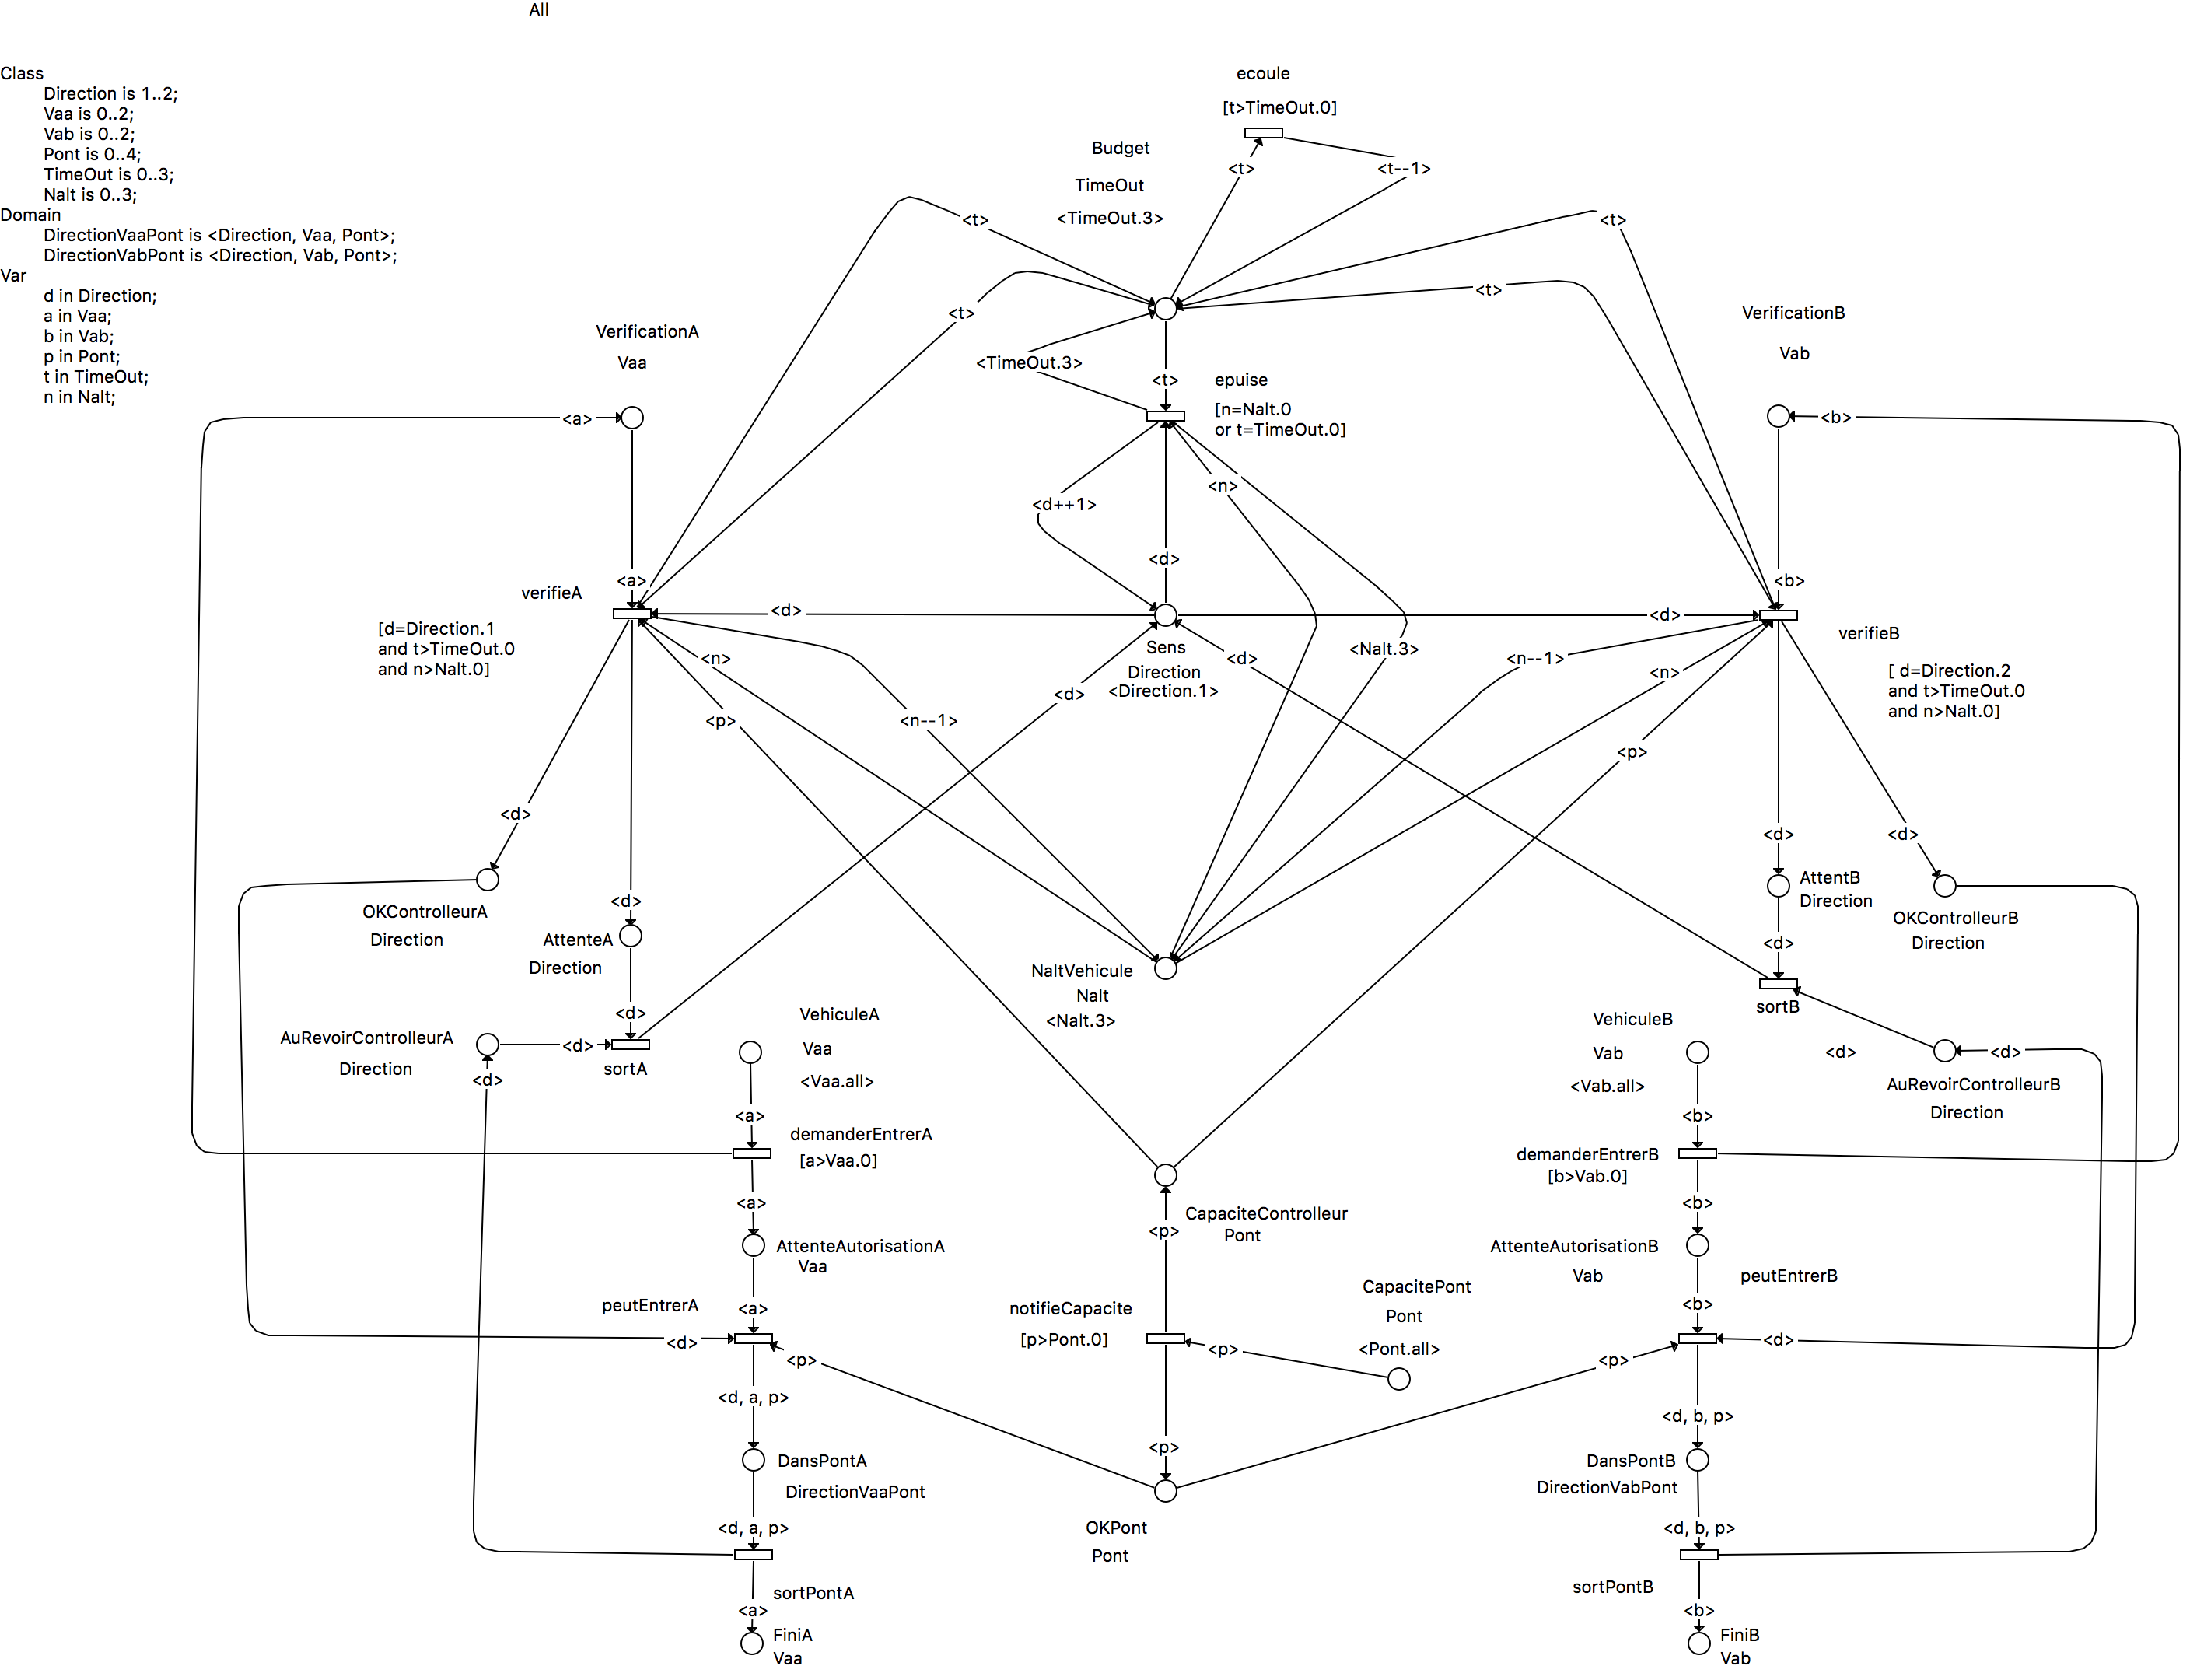
\includegraphics[width = 18cm]{allModel.png}
		\caption{Assemblage.}
	\end{figure}
	\newpage
	
\section{Question 1.7}
\subsubsection{Paramètres}
	Pour faciliter des vérifications car ma machine prend un temps énorme pour résoudre les formules. J'ai choisi:
	\begin{itemize}
		\item $N_{Vaa} = 2$
		\item $N_{Vab} = 2$
		\item $Capa_p = 4$
		\item $N_{Alt} = 3$
	\end{itemize}
	
	$Capa_p$ doit être supérieur au nombre total de véhicules, car sinon la propriété P2 ne peut être vérifiée.

\subsubsection{Vérification par CosyVerif4PN}
	Pour vérifier la propriété P1, \textit{"Il n'y a pas de collision (i.e. deux véhicules circulants en sens inverse) sur le pont."}, j'ai utilisé les formules suivantes:
	\begin{enumerate}
		\item \textit{query node ((card(DansPontA) + card(DansPontB)) == 2)}. Le résultat est zéro chemin. (Fichier P1\_1.txt)
		\item \textit{query node ((DansPontA == <.1.> and DansPontB == <.1.>) 
			\\or (DansPontA == <.1.> and DansPontB == <.2.>))}. Le résultat est zéro chemin. (Fichier P1\_2.txt)
		\item \textit{query node ((card(DansPontA) == 1) and (card(DansPontB) == 1))}. Le résultat est zéro chemin. (Fichier P1\_3.txt)
	\end{enumerate}
	
		Pour vérifier la propriété P2, \textit{"Un véhicule qui arrive est certain de passer sur le pont à l'issue d'une durée bornée."}, j'ai utilisé les formules suivantes:
		\begin{enumerate}
			\item \textit{query node (AG(implies(AttenteAutorisationA==<.1.>, AF(DansPontA:field[1]==<.1.>))))}. Le résultat est plusieurs chemins. (Fichier P2\_1.txt)
	\end{enumerate}
	
	Quelques formules pour les "autres propriétés triviales attendues":
		\begin{enumerate}
				\item \textit{query node ((card(VehiculeA) + card(AttenteAutorisationA) + card(DansPontA) + card(FiniA)) != 3)} : Le nombre de véhicules \textit{Vaa} reste constant. (Fichier P3\_1.txt et pour \textit{Vab} P3\_1Bis.txt)
				\item \textit{query node (card(CapacitePont) > 5)} : La capacité du pont $Capa_p$ est constante.(Fichier P3\_2.txt)
				\item \textit{query node (card(Budget) > 1)} : Il y a au plus 1 jeton dans la place \textbf{Budget} à la fois.(Fichier P3\_3.txt)
				\item \textit{query node (card(Sens) > 1)} : Il y a au plus 1 jeton dans la place \textbf{Sens} à la fois.(Fichier P3\_4.txt)
				\item \textit{query node (card(NaltVehicule) > 1)} : Il y a au plus 1 jeton dans la place \textbf{NaltVehicule} à la fois.(Fichier P3\_5.txt)
		\end{enumerate}
	
\section{Question 1.8}
	Ce problème ressemble comme l'exclusion mutuelle. Le contrôlleur est comme un serveur central, c'est lui qui gère les accès au pont. Il faut spécifier un protocol de communication entre le contrôlleur et les véhicules. Ensuite, il faut avoir des capteurs sur le pont pour calculer sa capacité restante. En plus, il faut assurer que les véhicules ne passent pas sur le pont sans autorisation du contrôlleur.
	
	En terme d'algorithmique répartie, ce modèle est comme le système client-serveur. Le timeout et le nombre de véhicules d'un même type sont bornés, le serveur peut gérer 2 files FIFO de demandes, 1 pour côté A et 1 pour côté B. La direction est changée régulièrement en un temps borné grâce au timeout et au nombre de véhicules d'un même type. Chaque véhicule qui sorte du pont doit signaler le contrôlleur. Donc, les 2 propriétés fondamentales du système sont vérifiées. Lorsque la capacité du pont atteint, le contrôlleur bloque tous les véhicules quelque soit leurs types.

\end{document}

